% !TEX TS-program = pdfLaTeX+shellescape
% !TEX encoding = UTF-8 Unicode

\documentclass{standalone}
\usepackage{pgfplots}
\pgfplotsset{compat=1.17}

\definecolor{tab_blue}{HTML}{1F77B4}
\definecolor{tab_green}{HTML}{2CA02C}
\definecolor{tab_red}{HTML}{D62728}

\begin{document}
    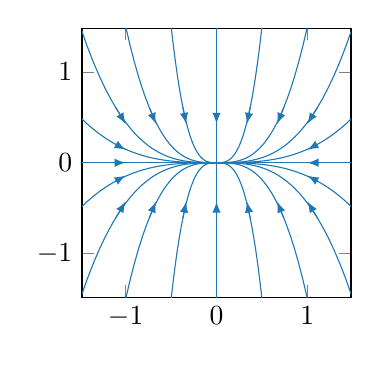
\begin{tikzpicture}[
        baseline,
        declare function = {
            solx(\a,\x) = \a*exp(-\x);
            soly(\b,\y) = \b*exp(-3*\y);
            derx(\a,\x) = -\a*exp(-\x);
            dery(\b,\y) = -3*\b*exp(-3*\y);
        }
        ]
        \begin{axis}[
            scale=0.6, % scale
            % view = {0}{90},
            xmin=-1.48,xmax=1.48,ymin=-1.48,ymax=1.48, % range of plot
            % legend style={at={(axis cs: 1,0)}, anchor=south east}, % position of legends
            % unit vector ratio = {1, 1, 1}, % aspect ratio
            unit vector ratio = {1, 1}, % aspect ratio
            % axis lines = box, % middle or box
            %axis x line = bottom, % top, middle, bottom, none: axis x line* = ... removes arrow heads
            %axis y line = left, % left, center, right, none: axis y line* = ... removes arrow heads
            %xlabel = {$x$}, ylabel = {$y$}, % axis labels 
        ]
            % \addplot[ultra thick, tab_green!75, domain=-1.5:1.5, samples=100]({x}, {0});
            % \addplot[ultra thick, tab_red!75, domain=-1.5:1.5, samples=100]({x}, {x});
            % \addplot[blue, domain=-1.5:1.5, samples=100]({x}, {0});
            \addplot[color=tab_blue, variable=\t, domain=0.0:5.0, samples=100]({solx(1.5, t)}, {soly(0.0, t)});
            \addplot[color=tab_blue, variable=\t, domain=0.0:5.0, samples=100]({solx(1.5, t)}, {soly(0.5, t)});
            \addplot[color=tab_blue, variable=\t, domain=0.0:5.0, samples=100]({solx(1.5, t)}, {soly(1.5, t)});
            \addplot[color=tab_blue, variable=\t, domain=0.0:5.0, samples=100]({solx(1.0, t)}, {soly(1.5, t)});
            \addplot[color=tab_blue, variable=\t, domain=0.0:5.0, samples=100]({solx(0.5, t)}, {soly(1.5, t)});
            \addplot[color=tab_blue, variable=\t, domain=0.0:5.0, samples=100]({solx(0.0,  t)}, {soly(1.5, t)});
            \addplot[color=tab_blue, variable=\t, domain=0.0:5.0, samples=100]({solx(-0.5, t)}, {soly(1.5, t)});
            \addplot[color=tab_blue, variable=\t, domain=0.0:5.0, samples=100]({solx(-1.0, t)}, {soly(1.5, t)});
            \addplot[color=tab_blue, variable=\t, domain=0.0:5.0, samples=100]({solx(-1.5, t)}, {soly(1.5, t)});
            \addplot[color=tab_blue, variable=\t, domain=0.0:5.0, samples=100]({solx(-1.5, t)}, {soly(0.5, t)});
            \addplot[color=tab_blue, variable=\t, domain=0.0:5.0, samples=100]({solx(-1.5, t)}, {soly(0.0, t)});
            \addplot[color=tab_blue, variable=\t, domain=0.0:5.0, samples=100]({solx(-1.5, t)}, {soly(-0.5, t)});
            \addplot[color=tab_blue, variable=\t, domain=0.0:5.0, samples=100]({solx(-1.5, t)}, {soly(-1.5, t)});
            \addplot[color=tab_blue, variable=\t, domain=0.0:5.0, samples=100]({solx(-1.0, t)}, {soly(-1.5, t)});
            \addplot[color=tab_blue, variable=\t, domain=0.0:5.0, samples=100]({solx(-0.5, t)}, {soly(-1.5, t)});
            \addplot[color=tab_blue, variable=\t, domain=0.0:5.0, samples=100]({solx(0.0, t)}, {soly(-1.5, t)});
            \addplot[color=tab_blue, variable=\t, domain=0.0:5.0, samples=100]({solx(0.5, t)}, {soly(-1.5, t)});
            \addplot[color=tab_blue, variable=\t, domain=0.0:5.0, samples=100]({solx(1.0, t)}, {soly(-1.5, t)});
            \addplot[color=tab_blue, variable=\t, domain=0.0:5.0, samples=100]({solx(1.5, t)}, {soly(-1.5, t)});
            \addplot[color=tab_blue, variable=\t, domain=0.0:5.0, samples=100]({solx(1.5, t)}, {soly(-0.5, t)});
            
            % arrow
            \addplot[color=tab_blue, variable=\t, samples=2, domain=-1.0:0.3, -latex, quiver={u={derx(1.5, t)}, v={dery(0.0, t)}, scale arrows=0.1}]({solx(1.5, t)}, {soly(0.0, t)});
            \addplot[color=tab_blue, variable=\t, samples=2, domain=-1.0:0.3, -latex, quiver={u={derx(1.5, t)}, v={dery(0.5, t)}, scale arrows=0.1}]({solx(1.5, t)}, {soly(0.5, t)});
            \addplot[color=tab_blue, variable=\t, samples=2, domain=-1.0:0.3, -latex, quiver={u={derx(1.5, t)}, v={dery(1.5, t)}, scale arrows=0.1}]({solx(1.5, t)}, {soly(1.5, t)});
            \addplot[color=tab_blue, variable=\t, samples=2, domain=-1.0:0.3, -latex, quiver={u={derx(1.0, t)}, v={dery(1.5, t)}, scale arrows=0.1}]({solx(1.0, t)}, {soly(1.5, t)});
            \addplot[color=tab_blue, variable=\t, samples=2, domain=-1.0:0.3, -latex, quiver={u={derx(0.5, t)}, v={dery(1.5, t)}, scale arrows=0.1}]({solx(0.5, t)}, {soly(1.5, t)});
            \addplot[color=tab_blue, variable=\t, samples=2, domain=-1.0:0.3, -latex, quiver={u={derx(0.0, t)}, v={dery(1.5, t)}, scale arrows=0.1}]({solx(0.0, t)}, {soly(1.5, t)});
            \addplot[color=tab_blue, variable=\t, samples=2, domain=-1.0:0.3, -latex, quiver={u={derx(-0.5, t)}, v={dery(1.5, t)}, scale arrows=0.1}]({solx(-0.5, t)}, {soly(1.5, t)});
            \addplot[color=tab_blue, variable=\t, samples=2, domain=-1.0:0.3, -latex, quiver={u={derx(-1.0, t)}, v={dery(1.5, t)}, scale arrows=0.1}]({solx(-1.0, t)}, {soly(1.5, t)});
            \addplot[color=tab_blue, variable=\t, samples=2, domain=-1.0:0.3, -latex, quiver={u={derx(-1.5, t)}, v={dery(1.5, t)}, scale arrows=0.1}]({solx(-1.5, t)}, {soly(1.5, t)});
            \addplot[color=tab_blue, variable=\t, samples=2, domain=-1.0:0.3, -latex, quiver={u={derx(-1.5, t)}, v={dery(0.5, t)}, scale arrows=0.1}]({solx(-1.5, t)}, {soly(0.5, t)});
            \addplot[color=tab_blue, variable=\t, samples=2, domain=-1.0:0.3, -latex, quiver={u={derx(-1.5, t)}, v={dery(0.0, t)}, scale arrows=0.1}]({solx(-1.5, t)}, {soly(0.0, t)});
            \addplot[color=tab_blue, variable=\t, samples=2, domain=-1.0:0.3, -latex, quiver={u={derx(-1.5, t)}, v={dery(-0.5, t)}, scale arrows=0.1}]({solx(-1.5, t)}, {soly(-0.5, t)});
            \addplot[color=tab_blue, variable=\t, samples=2, domain=-1.0:0.3, -latex, quiver={u={derx(-1.5, t)}, v={dery(-1.5, t)}, scale arrows=0.1}]({solx(-1.5, t)}, {soly(-1.5, t)});
            \addplot[color=tab_blue, variable=\t, samples=2, domain=-1.0:0.3, -latex, quiver={u={derx(-1.0, t)}, v={dery(-1.5, t)}, scale arrows=0.1}]({solx(-1.0, t)}, {soly(-1.5, t)});
            \addplot[color=tab_blue, variable=\t, samples=2, domain=-1.0:0.3, -latex, quiver={u={derx(-0.5, t)}, v={dery(-1.5, t)}, scale arrows=0.1}]({solx(-0.5, t)}, {soly(-1.5, t)});
            \addplot[color=tab_blue, variable=\t, samples=2, domain=-1.0:0.3, -latex, quiver={u={derx(0.0, t)}, v={dery(-1.5, t)}, scale arrows=0.1}]({solx(0.0, t)}, {soly(-1.5, t)});
            \addplot[color=tab_blue, variable=\t, samples=2, domain=-1.0:0.3, -latex, quiver={u={derx(0.5, t)}, v={dery(-1.5, t)}, scale arrows=0.1}]({solx(0.5, t)}, {soly(-1.5, t)});
            \addplot[color=tab_blue, variable=\t, samples=2, domain=-1.0:0.3, -latex, quiver={u={derx(1.0, t)}, v={dery(-1.5, t)}, scale arrows=0.1}]({solx(1.0, t)}, {soly(-1.5, t)});
            \addplot[color=tab_blue, variable=\t, samples=2, domain=-1.0:0.3, -latex, quiver={u={derx(1.5, t)}, v={dery(-1.5, t)}, scale arrows=0.1}]({solx(1.5, t)}, {soly(-1.5, t)});
            \addplot[color=tab_blue, variable=\t, samples=2, domain=-1.0:0.3, -latex, quiver={u={derx(1.5, t)}, v={dery(-0.5, t)}, scale arrows=0.1}]({solx(1.5, t)}, {soly(-0.5, t)});
            
        \end{axis}
    \end{tikzpicture}
\end{document}